% AOSD report template
% Valentino Vranić 2018

\documentclass[11pt,english,a4paper,twoside]{article}
%\documentclass[11pt,slovak,a4paper,twoside]{article}

\usepackage[IL2]{fontenc}

\usepackage[utf8]{inputenc}
\usepackage{babel}
\usepackage{url}
\usepackage[nottoc]{tocbibind}
\usepackage{ifthen}
\usepackage[hidelinks]{hyperref}
\usepackage{graphicx}
\usepackage{listings}
\usepackage{verbatim}
\usepackage{float}
\lstset{language=[AspectJ]Java,basicstyle=\fontsize{9}{10.8}\selectfont,showstringspaces=false,columns=fullflexible}

\newcommand{\magnf}{.65}
\newcommand{\codesize}{\footnotesize}
\newcommand{\lsti}{\ajset\lstinline[basicstyle=\fontsize{10}{12}\selectfont]}
\newcommand{\emp}[1]{\emph{#1}}
\newcommand{\ffe}[1]{\textsf{#1}}

% balík listings niekedy niektoré kľúčové slová nezvýrazňuje ak to nedostane príkazom tesne pred textom
\newcommand{\ajset}{\lstset{emph={class,aspect,new,call,execution,set,int,advice,public,thisJoinPointStaticPart,thisEnclosingJoinPointStaticPart,@annotation,dominates},emphstyle=\bfseries}}

\newcommand{\reporttitle}{Data versioning in machine-learning architecture}
% here goes your fancy title

\pagestyle{myheadings}
\markboth{\reporttitle}{Software Architecture 2024/25, FIIT STU}

\title{\reporttitle}

\author{Peter Bartoš, Stanislav Krištof} % your name

\date{Faculty of Informatics and Information Technologies\\
      Slovak University of Technology in Bratislava\\[6pt]
      \today}



\begin{document}

\maketitle

\begin{abstract}
Data versioning plays a crucial role in modern machine learning architecture,
ensuring that the complex and ever-evolving datasets that provide the basis for
models can be tracked, compared, and managed efficiently. At its core, data
versioning refers to the practice of creating unique references for different
states of a dataset over time, allowing us to trace changes, restore previous
versions, and debug issues. This is vital in machine learning workflows, where
even small changes in data can significantly impact model performance.

In this domain, data versioning supports reproducibility by maintaining a
consistent link between datasets and the models trained on them. Without version
control, it becomes challenging to recreate experiments, leading to
inconsistencies in predictions and hindering model audits. Versioning also
simplifies collaboration across teams, enabling multiple stakeholders to work on
the same data without overwriting each other's progress.

Basic approaches to data versioning systems (DVS) include full duplication of
datasets, where copies are saved with each change, and metadata-based
versioning, where timestamps indicate the validity of each record. Advanced
solutions (like lakeFS and DVC) deal with versioning as a core component of
machine learning architecture. They enable storage-efficient data commits,
branching, and comparison, similar to how Git handles version control in
software development.

Overall, data versioning enhances productivity, reduces errors, and fosters an
engineering-driven approach to handling data in machine learning pipelines,
ultimately enabling smoother transitions between development stages and more
robust model deployment. The objective of the project is to go over these
systems and provide detailed overviews of how data versioning has such a crucial
role in machine learning architecture.
\end{abstract}


\section{Introduction} \label{in}

%\ldots

Reproducibility, as defined by ACM \cite{ACMreproducibility}, 
is the ability to obtain precise measurements by different 
teams under the same conditions. In AI advancements, reproducibility 
is crucial, with Peng \cite{peng2011reproducible} considering it 
the ultimate measure of scientific validity. However, Pawlik et 
al. \cite{pawlik2019link} found that only 7.64\% of analyzed papers 
were reproducible. Improved data version control can enhance 
reproducibility and enable more complex studies, increasing understanding 
of neural networks. Pawlik et al. \cite{pawlik2019link} suggest that 
datasets should include not only input data but also raw data and 
preparation instructions to improve context and reproducibility. 
\\\\
To understand how data versioning integrates into machine learning 
architecture, it's essential to examine key components and workflows. 
Machine learning pipelines rely on iterative experimentation, where 
data is critical at every stage, from preprocessing to model training, 
evaluation, and deployment. Maintaining consistent, traceable versions 
of datasets and models is vital for ensuring reproducibility. 
\cite{wandb}
\paragraph{Outlook}
The rest of this report is structured as follows. Section~\ref{insight} provides
an insight into\ldots{} Section~\ref{approaches} explains in more detail some
important approaches to\ldots{} Section~\ref{initial} brings the initial steps
to\ldots{} (Characterize each section by a sentence.) Section~\ref{cc}
concludes the paper and indicates some directions for further work.



\section{Insight into\ldots} \label{insight}
\paragraph{Types of Data Version Control Systems (DVCS)}
According to Zolkifli et al. \cite{zolkifli2018version} in centralised DVCS, a
singular repository is located on the server. These DVCS are suitable for teams
with smaller number of members, with the team being located in a single place.
Only the last version of a file is retrieved and there is a single point of
failure. Examples include Apache Subversion or Perforce Revision Control System.
In distributed DVCS, on the other hand, each user has one local repository.
Examples include Git, Mercurial, Bazaar or Bitkeeper. This type is suitable
regardless of team size. It also enables users being located in different parts
of the world. Clients can create their own branches and sync them with the
server.
\paragraph{Git}
As stated by Komsiyski \cite{komsiyski2013binary}, Git works on basis of patch
files. As noted by Bryan \cite{bryan2018excuse}, large and often changing files
are not suitable for Git, since they can slow down pushes and pulls. According
to Perez et al. \cite{perez2016ten}, binary files in git are stored as a single
large entity. Therefore, even small changes lead to new copies in the
repository. This also makes it difficult to compare changes in files using diff
and may lead to frequent merge conflicts.

\paragraph{Git LFS}
Git also offers an extension for large files called Git LFS (Large File
Storage), which enables more efficient handling of large files
\cite{perez2016ten}. Content of the file is stored in cloud, with the repository
containing only pointers to the files, as noted in the documentation
\cite{gitlfs-structure} (Figure \ref{fig:gitlfs-architecture}). Since Git LFS is
a GitHub extension, its advantages are compatibility with Git
\cite{gitlfs-collaboration} and file agnosticism (compatibility with all file
formats) \cite{comparison}. Its disadvantages are inefficient storage management
- similar to Git, edited files are stored as new files. Therefore, it is not
suitable for large frequently-changing files, especially if they are compressed
(such as file formats frequently used in computer vision, e.g. jpg, png)
\cite{git-lfs}. In addition, data in Git LFS do not stay in place. It also does
not scale as well and its data retrieval is slow. As such, this approach is
suitable mostly for game developers and not for for ML and data science
purposes.

\begin{figure}[H]
    \centering
    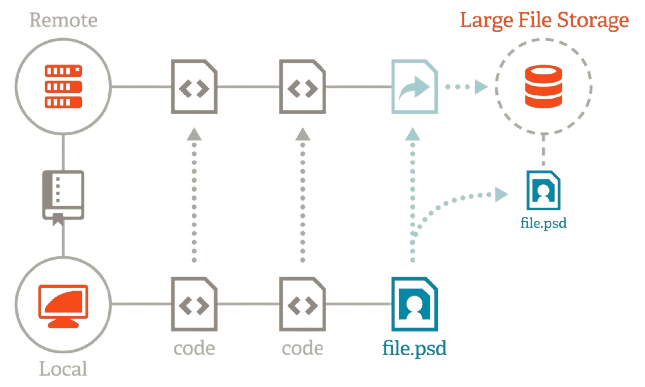
\includegraphics[width=0.8\textwidth]{fig/gitlfs-arch.png}
    \caption{Software architecture of Git LFS \cite{gitlfs-architecture}}
    \label{fig:gitlfs-architecture}
\end{figure}

\begin{comment}
Git offers a Large File Storage (LFS) module that
replaces such large files with pointers while the large binary file can be
stored remotely, which results in smaller and faster repositories. Git LFS is
also supported by GitHub, albeit with a space quota or for a fee, to retain your
usual GitHub workflow (https://help.github.com/categories/managing-large-files/)
(S1 File, Section 1).

GIT LFS (Large File Storage)

files above 50mb should be commited using Git LFS. 1 GiB of storage is free for
every account, together with 1GiB bandwidth. 5$ = 50 GiB storage, 50 GiB
bandwidth. text pointers are stored in git, the actual binary files are on cloud


https://www.atlassian.com/git/tutorials/git-lfs
https://docs.github.com/en/repositories/working-with-files/managing-large-files/about-storage-and-bandwidth-usage

When you commit and push a change to a file tracked with Git LFS, a new version
of the entire file is pushed and the total file size is counted against the
repository owner's storage limit. When you download a file tracked with Git LFS,
the total file size is counted against the repository owner's bandwidth limit.
Git LFS uploads do not count against the bandwidth limit.

For example:

If you push a 500 MB file to Git LFS, you'll use 500 MB of your allotted storage
and none of your bandwidth. If you make a 1 byte change and push the file again,
you'll use another 500 MB of storage and no bandwidth, bringing your total usage
for these two pushes to 1 GB of storage and zero bandwidth. If you download a
500 MB file that's tracked with LFS, you'll use 500 MB of the repository owner's
allotted bandwidth. If a collaborator pushes a change to the file and you pull
the new version to your local repository, you'll use another 500 MB of
bandwidth, bringing the total usage for these two downloads to 1 GB of
bandwidth. If GitHub Actions downloads a 500 MB file that is tracked with LFS,
it will use 500 MB of the repository owner's allotted bandwidth.
git works on basis of patch files, as Komsiyski states

\cite{komsiyski2013binary}, time for creating a patch and sending the patch to a
server has to be less than the time needed to send a new version of file to the
server.
\end{comment}
\paragraph{Dolt}
Dolt is a version-controlled SQL database and as such it may serve as an example
of a centralised DVS. Analogous to Git, one can track schemas and changes in the
database, create and merge branches \cite{dolt-reproducibility}. Under the hood,
Dolt uses Prolly trees - a data structure related to both B-trees
\cite{prolly-trees}, commonly used in RDBMS and Merkle trees (used by
distributed version control systems such as Git or Mercurial)\cite{comparison}.
This data structure provides both fast performance (including diffs and merges)
and efficient storage management (each portion of data shared between trees is
shared only once). However, like other RDBMS, while Dolt may be the ideal
solution for structured data, it is not suitable for unstructed data.
\begin{comment}
    version controlled SQL DB; suitable for data stored in RDBMS (such as MySQL,
although there appears to be a postgres version as well) usage of prolly trees
(merge of B-tree (indices of RDBMS, performance of databases) and Merkle tree
(structure used in git)) = data is saved in accordance to hash (easier
identification whether file changed, better diff / merge);not suitable for
unstructured data, nor high performance; centralised; tracking of schemas and
changes in the database ;(source: github read me file);
https://docs.dolthub.com/introduction/use-cases = overview of usecases not great
for unstructured binary files; can effectively serve to replace databases;
support merging, branching and other typical git stuff;
\end{comment}
\paragraph{DVC by Iterative}
Another solution, suitable for ML learning may be DVC \cite{DVC}. DVC achieves
faster data retrieval by its data staying in place. In addition, DVC also uses a
caching layer (Figure \ref{fig:dvc-architecure}), which allows faster data
retrieval for multiple members of team \cite{comparison}. DVC supports both
structured and unstructed data. It however does not support RDBMS. Since it
caters to data scientists, it offers several features which greatly lead to
higher reproducibility, such as defining data pipelines
\cite{dvc-define-pipelines}, visualisation of pipelines
\cite{dvc-run-pipelines}, experiment tracking \cite{dvc-compare-experiments} and
hydra compatibility \cite{dvc-hydra}. It also does not scale as well, mostly due
to the same reasons as git.

\begin{figure}[H]
    \centering
    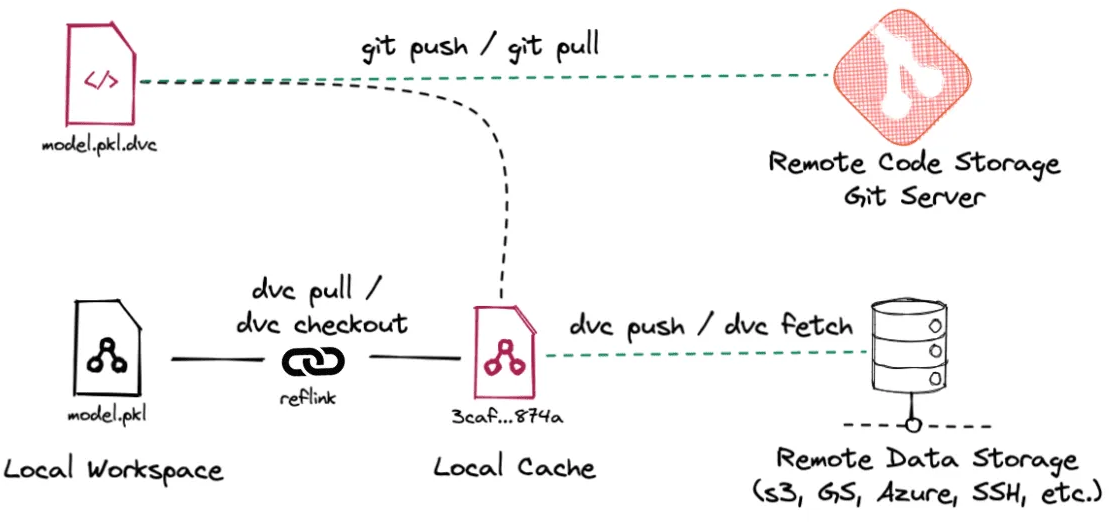
\includegraphics[width=0.8\textwidth]{fig/dvc-arch.png}
    \caption{Software architecture of DVC \cite{comparison}}
    \label{fig:dvc-architecture}
\end{figure}

\begin{comment}
Iterative offers DVC \cite{DVC}, which allows users to save and track model data
and models. Data and models are captured using git commits and can be stored
both locally or in cloud. DVC works by creating metafiles, that describe data to
be tracked. metafiles are put in Git instead of large files.
\end{comment}
Present your insight into the state of the art.
Favor comparison and critique over description.
Avoid lengthy descriptions with lots of quoted material.

Use your own title for this section..

You may structure your sections (see below).
If you use subsections, use at least two, i.e., don't put only one subsection.

It might be a good idea to explain the structure of the rest of the section.
Sometimes, an explicit way of doing at just as is demonstrated at the end of the
introduction (see Section~\ref{in}).


\subsection{Some Aspects} \label{insight-some}

\ldots

\subsection{Other Aspects} \label{insight-other}

\ldots



\section{Important Approaches to\ldots} \label{approaches}

You may need one more section to treat the state of the art.
Everything said for the previous section, holds for this one, too.




\section{Initial Steps to\ldots} \label{initial}

Describe your own approach.
Of course, use your own title for this section.

Put your diagrams in figures as so-called floating object.
Refer to them using their numbers.
E.g., ``in Figure~\ref{f:gen-spec} we can see\ldots''

\begin{figure}[tbh] \centering
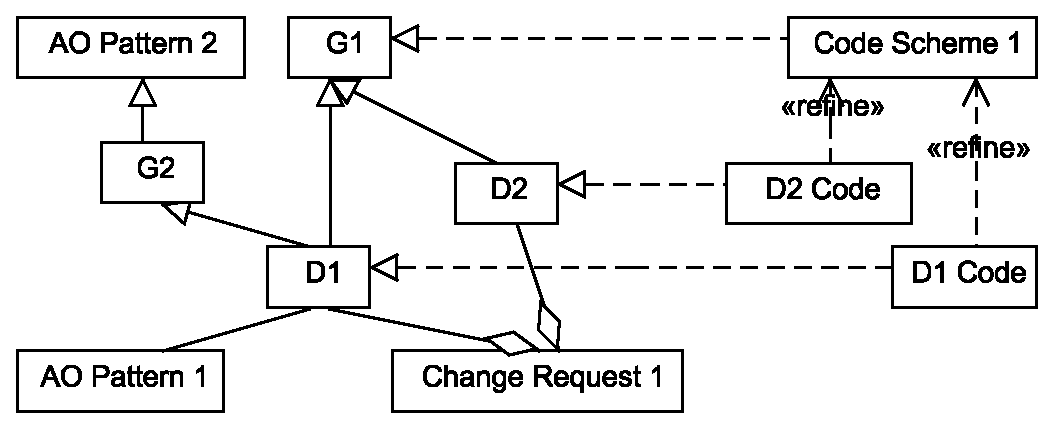
\includegraphics[scale=\magnf]{fig/gen-spec}
\caption{Generally applicable and domain specific changes.}
\label{f:gen-spec}
\end{figure}


You may include code snippets to explain what you've done:
\ajset
\begin{lstlisting}
public class SMTPServerM extends SMTPServer {
   . . .
}
. . .
public aspect SMTPServerBackupA {
   public pointcut SMTPServerConstructor(URL url, String user, String password):
      call(SMTPServer.new(..)) && args (url, user, password);
   SMTPServer around(URL url, String user, String password):
      SMTPServerConstructor(url, user, password) {
      return getSMTPServerBackup(proceed(url, user, password));
   }
   private SMTPServer getSMTPServerBackup(SMTPServer obj) {
      if (obj.isConnected()) {
         return obj;
      }
      else {
         return new SMTPServerM(obj.getUrl(), obj.getUser(),
            obj.getPassword());
      }
   }
}
\end{lstlisting}

If you need to display more code, use appendices referring the reader to them,
e.g., ``see Appendix~\ref{some} for a more detailed example.''



\section{Further Steps to\ldots} \label{further}

You may need several sections to describe your approach.



\section{Evaluation} \label{eval}

You may describe your evaluation efforts in a separate, often generically
entitled section.

\subsection{Essential Evaluation} \label{eval-essential}

Use your own title here.

\subsection{Threats to Validity} \label{eval-threats}

\ldots



\section{Related Work} \label{rw}

Compare your achievements to related ones achieved by others.



\section{Conclusions and Further Work} \label{cc}

% Conclusions
Emphasize the main results.

% Further Work
Indicate what can be done next.

The concluding section is typically not decomposed into subsections.
Simply use several paragraphs to present conclusions,
and then use at least one paragraph to indicate further/future work.


\bibliographystyle{abbrv} % plain or alpha are fine, too
\bibliography{bib}

\appendix
\section{Some Appendix} \label{some}


\section{Yet Another Appendix} \label{yetanother}


\end{document}

